\documentclass[10pt,twocolumn,a4paper]{article}
\usepackage[margin=1.75cm,top=2.0cm,bottom=2.0cm,columnsep=0.65cm]{geometry}
\usepackage{amsmath,amssymb,amsfonts}
\usepackage{graphicx}
\graphicspath{{figures/}{../figures/}}
\usepackage{booktabs}
\usepackage{xcolor}
\usepackage{fancyhdr}
\usepackage{caption}
\usepackage{subcaption}
\usepackage{hyperref}
\usepackage{array}
\usepackage{tikz}
\usetikzlibrary{shapes,arrows,positioning,calc}

% Avoid textcomp font dependencies for bullets
\renewcommand{\labelitemi}{$\bullet$}
\renewcommand{\labelitemii}{$\circ$}
\renewcommand{\labelitemiii}{$\ast$}
\renewcommand{\labelitemiv}{$\cdot$}

\hypersetup{
    colorlinks=true,
    linkcolor=blue!80!black,
    citecolor=blue!80!black,
    urlcolor=blue!80!black,
    pdftitle={Fine-Grained Emotion Classification in Social Media Text: A Comparative Study of Classical Ensembles and Deep Sequence Models Under Class Imbalance},
    pdfauthor={Nishant Kumar}
}

\pagestyle{fancy}
\fancyhf{}
\fancyhead[L]{\footnotesize\textit{Fine-Grained Emotion Classification in Social Media Text}}
\fancyhead[R]{\footnotesize\textit{Nishant Kumar}}
\fancyfoot[C]{\thepage}
\renewcommand{\headrulewidth}{0.4pt}

\title{\vspace{-0.6cm}\LARGE\textbf{Fine-Grained Emotion Classification in Social Media Text:\\A Comparative Study of Classical Ensembles and Deep Sequence Models Under Class Imbalance}}

\author{
    \textbf{Nishant Kumar}\\
    Department of Artificial Intelligence \& Machine Learning\\
    \url{https://github.com/nishantkumar-AIML/sentiment}
}
\date{\today}

\begin{document}

\maketitle

\begin{abstract}
Automated fine-grained emotion recognition in social media microblogs is a critical prerequisite for mental health monitoring, conversational AI, empathetic customer support, and disaster informatics. Unlike coarse binary or ternary sentiment analysis, multi-class emotion classification requires discriminating between subtle affective states with overlapping lexical features and acute class distribution skews. In this study, we present a rigorous, controlled comparative evaluation of six distinct machine learning paradigms (Multinomial Logistic Regression, Linear Support Vector Machines, Random Forest, Multinomial Naive Bayes, Extreme Gradient Boosting [XGBoost], and Bidirectional LSTM Neural Networks) for six-class emotion classification (\textit{Sadness}, \textit{Joy}, \textit{Love}, \textit{Anger}, \textit{Fear}, \textit{Surprise}). Operating on a standardized 20,000-sample English Twitter corpus, we execute an explicit cross-split data leakage audit, identifying 16 training instances that overlapped with validation or test texts, which were removed from the training split to establish a strictly isolated 15,984-sample clean training set. Our experimental results reveal pivotal methodological findings: Linear Support Vector Machine achieves the highest overall accuracy of \textbf{88.40\%} (Macro-F1 = \textbf{0.8312}), while XGBoost achieves the highest balanced Macro-F1 of \textbf{0.8332} (Accuracy = \textbf{87.50\%}), closely followed by Random Forest (\textbf{87.25\%} Accuracy, Macro-F1 = \textbf{0.8208}) and Multinomial Logistic Regression (\textbf{85.00\%} Accuracy, Macro-F1 = \textbf{0.7724}). Crucially, the minority emotion \textit{Surprise} (representing only 3.57\% of the clean training set) suffers severe performance degradation across classical baselines and exhibits acute sensitivity in the baseline 3-epoch PyTorch Bi-LSTM (F1 = 0.1096, Overall Accuracy = 80.70\%, Macro-F1 = 0.6372), underscoring the sample-efficiency challenge of optimizing randomly initialized neural embeddings and recurrent weights from scratch under class scarcity. Exploratory diagnostic ablation studies establish that stopword filtering yields a notable improvement over raw unigrams (P2: 88.95\% Accuracy, Macro-F1 = 0.8367; P3: 88.90\% Accuracy, Macro-F1 = 0.8360), while class-weighted loss increases Macro-F1 to \textbf{0.8452}, and targeted TF-IDF synthetic oversampling produces a Macro-F1 of \textbf{0.8456} and \textit{Surprise} F1 of \textbf{0.7133}. We provide a complete open-source reproducibility package to facilitate transparent benchmarking.
\vspace{0.6em}

\noindent \textbf{\textit{Keywords}}---Natural Language Processing, Fine-Grained Emotion Recognition, Multi-Class Text Classification, Linear SVM, XGBoost, Random Forest, Bidirectional LSTM, Class Imbalance, Macro-F1 Evaluation, Data Leakage Prevention, Reproducibility.
\end{abstract}

\section{Introduction}
\label{sec:intro}

The explosive growth of social media platforms has established microblogging services as principal digital repositories of human opinions, affective expressions, and psychosocial dynamics. Mining subjective sentiment from these unstructured streams has historically focused on coarse-grained polarity classification, distinguishing between positive, negative, and neutral polarities~\cite{qi2023sentiment, bhardwaj2020sentiment}. However, modern applications---ranging from real-time psychiatric triage and suicide risk detection to conversational AI, empathetic customer support, and disaster informatics---require a far more granular understanding of discrete human emotional states~\cite{saravia2018carer, demszky2020goemotions, mutanov2021multiclass}.

Fine-grained emotion classification extends conventional polarity analysis by categorizing texts into discrete psychological categories derived from foundational affect theories, such as Ekman's primary emotions (\textit{Sadness}, \textit{Joy}, \textit{Anger}, \textit{Fear}, \textit{Surprise}) augmented with complex interpersonal states such as \textit{Love}~\cite{saravia2018carer, khandagale2025sentiment}. Despite its utility, fine-grained text emotion classification presents severe computational and linguistic challenges:
\begin{enumerate}
    \item \textbf{Semantic Proximity and Boundary Ambiguity}: Emotions within the same valence domain (e.g., \textit{Joy} and \textit{Love}, or \textit{Anger} and \textit{Fear}) often share syntactic structures, emotive vocabulary, and contextual patterns, leading to substantial inter-class confusion.
    \item \textbf{Informal Text Noise}: Social media posts are characterized by irregular grammar, non-standard orthography, slang, abbreviations, and implicit emotional cues that lack explicit affect lexicons.
    \item \textbf{Acute Class Imbalance}: In organic social media communication, emotions such as \textit{Joy} and \textit{Sadness} occur with vastly higher frequency than low-base-rate emotions such as \textit{Surprise} or \textit{Love}, creating skewed class distributions that severely penalize minority class recall.
\end{enumerate}

\subsection{Research Gaps \& Motivation}
While numerous studies report high aggregate accuracy on emotion datasets, recent reproducibility and methodological literature highlights critical flaws in standard text classification pipelines~\cite{pmc11948487_reproducibility}:
\begin{itemize}
    \item \textit{The Accuracy Illusion}: Relying solely on overall accuracy obscures catastrophic failure modes on minority classes, where a model can achieve $>85$\% accuracy simply by predicting majority classes.
    \item \textit{Data Leakage and Duplicate Ingestion}: Many public benchmarks suffer from undocumented cross-split sample overlap between training, validation, and testing sets, artificially inflating reported performance.
    \item \textit{Sparse Feature vs. Sequential Trade-offs}: It remains contentious whether modern recurrent neural sequence architectures (such as Bi-LSTMs) consistently outperform classical, regularized feature-engineered algorithms (such as XGBoost and Linear SVM) when operating under standard data regimes without billions of pre-trained parameters.
\end{itemize}

\subsection{Research Questions and Hypotheses}
To resolve these open challenges, this study addresses five fundamental research questions:
\begin{itemize}
    \item \textbf{RQ1}: How do linear, probabilistic, and tree-based ensemble algorithms compare for six-class emotion recognition using identical TF-IDF vector space representations?
    \item \textbf{RQ2}: Does Macro-F1 produce a divergent model ranking compared to overall accuracy under acute multi-class imbalance?
    \item \textbf{RQ3}: How does a Bidirectional LSTM sequence model compare against sparse classical classifiers under equivalent dataset splits?
    \item \textbf{RQ4}: Which specific emotional classes exhibit the highest classification resistance, and what linguistic mechanisms drive cross-class error?
    \item \textbf{RQ5}: What feature engineering, preprocessing, and class-balancing strategies most effectively alleviate minority-class degradation?
\end{itemize}

\noindent We formulate the following testable scientific hypotheses:
\begin{itemize}
    \item \textbf{H1}: Non-linear gradient boosted tree ensembles (XGBoost) will achieve top-tier Macro-F1 by modeling non-linear feature interactions across emotive tokens.
    \item \textbf{H2}: Macro-F1 will rank models differently than overall accuracy, favoring classifiers with robust decision boundaries on minority emotions.
    \item \textbf{H3}: The extreme minority class (\textit{Surprise}) will suffer the lowest F1-score across all candidate architectures.
    \item \textbf{H4}: Recurrent sequence architectures trained from scratch with randomly initialized embeddings will exhibit acute sensitivity and lower minority-class recall under constrained training budgets due to limited gradient updates on low-support classes.
\end{itemize}

\subsection{Principal Contributions}
The key contributions of this paper are summarized as follows:
\begin{enumerate}
    \item \textbf{Rigorous Data Audit \& Leakage Remediation}: We perform a complete cross-split duplicate audit on the 20,000-sample emotion corpus, identifying and removing 16 cross-split overlapping instances to establish a strictly isolated 15,984-instance training set.
    \item \textbf{Comprehensive Multi-Model Benchmarking}: We conduct a controlled empirical evaluation across six standard model paradigms: Multinomial Logistic Regression, Linear SVM, Random Forest (100 trees), Multinomial Naive Bayes, XGBoost (100 estimators), and a PyTorch-based Bidirectional LSTM.
    \item \textbf{Metric-Dependent Model Comparison}: In our experimental setting, the accuracy and Macro-F1 rankings differed between the top two models: Linear SVM achieved the highest overall accuracy (\textbf{88.40\%}), whereas XGBoost achieved the highest Macro-F1 (\textbf{0.8332}), illustrating the practical importance of evaluating multi-class imbalance with both aggregate and unweighted metrics.
    \item \textbf{Neural Sequence Convergence Analysis}: We diagnose and quantify the minority-class representation sensitivity in low-epoch Bi-LSTM networks, offering theoretical and empirical explanations for why sparse linear and tree models outperform recurrent baselines in this setting.
    \item \textbf{Systematic Ablation and Error Taxonomy}: We execute feature-size scaling, n-gram expansion, preprocessing ablation, and compile a 5-part qualitative linguistic error taxonomy.
    \item \textbf{Full Open-Science Reproducibility}: We release our end-to-end Python pipeline, configurations, and canonical experiment results in a public repository\footnote{\url{https://github.com/nishantkumar-AIML/sentiment}}.
\end{enumerate}

% ------------------------------------------------------------
\section{Related Work}
\label{sec:related_work}

Text affect recognition has evolved across three major methodological eras: lexicon-based systems, classical feature-engineered machine learning, and deep neural architectures.

\subsection{Lexicon- and Rule-Based Methods}
Early emotion detection relied heavily on curated linguistic lexicons, such as the NRC Emotion Lexicon~\cite{mohammad2013crowdsourcing}, LIWC~\cite{pennebaker2001linguistic}, and VADER~\cite{hutto2014vader}. These systems compute aggregate emotional valence by matching input tokens against predetermined affect weights. While highly interpretable and computationally lightweight, lexicon-based approaches fail catastrophically when encountering sarcasm, negation shifts, polysemy, and colloquial social media syntax, as demonstrated in recent comparative evaluations by Qi and Shabrina~\cite{qi2023sentiment}.

\subsection{Classical Machine Learning \& Feature Extraction}
The application of supervised machine learning algorithms transformed text classification by learning discriminative decision boundaries directly from labeled corpora~\cite{mutanov2021multiclass, bhardwaj2020sentiment}. Term Frequency-Inverse Document Frequency (TF-IDF) and Bag-of-Words (BoW) remain robust, gold-standard sparse representations for microblog mining~\cite{qi2023sentiment}. 

Mutanov et al.~\cite{mutanov2021multiclass} evaluated Naive Bayes, Support Vector Machines (SVM), Logistic Regression, k-Nearest Neighbors (k-NN), Decision Trees, Random Forests, and XGBoost on multi-class social media text, observing that tree ensembles and SVMs consistently outperform probabilistic baselines. Similarly, Bhardwaj~\cite{bhardwaj2020sentiment} demonstrated that linear SVMs paired with n-gram TF-IDF features achieve strong classification bounds on noisy web text. However, existing classical literature frequently overlooks the divergence between overall accuracy and macro-averaged metrics under acute class imbalance.

\begin{table*}[t]
\centering
\small
\caption{Structured Literature Matrix: Comparative Analysis of Prior Emotion \& Sentiment Studies vs. Our Work.}
\label{tab:literature_matrix}
\resizebox{\textwidth}{!}{
\begin{tabular}{lp{2.0cm}p{2.2cm}cp{2.4cm}p{3.2cm}ccp{2.8cm}}
\toprule
\textbf{Study} & \textbf{Venue / Year} & \textbf{Domain / Data} & \textbf{Classes} & \textbf{Features / Repr.} & \textbf{Models Evaluated} & \textbf{Best Metric} & \textbf{Leakage Audit?} & \textbf{Primary Identified Limitation} \\
\midrule
Qi \& Shabrina~\cite{qi2023sentiment} & SNAM 2023 & Twitter Posts & 3 & BoW, TF-IDF, W2V & Lexicon, NB, SVM, LR & 78.4\% Acc & No & Coarse 3-class only; no neural baselines. \\
Mutanov et al.~\cite{mutanov2021multiclass} & CMC 2021 & Social Media & 3 & TF-IDF, Count & NB, SVM, LR, RF, XGB & 83.2\% Acc & No & Class imbalance treated primarily via SMOTE. \\
Bhardwaj~\cite{bhardwaj2020sentiment} & ISMAC 2020 & Social Web Text & 3 & TF-IDF, N-grams & SVM, NB, Decision Tree & 74.6\% Acc & No & Small dataset size; no deep sequence models. \\
Khandagale \& Kumar~\cite{khandagale2025sentiment} & IJISAE 2025 & Social Media & 6 & Word Embeddings & CNN, LSTM, BERT & 86.2\% Acc & No & High computational overhead; no classical ablation. \\
Saravia et al.~\cite{saravia2018carer} & EMNLP 2018 & Twitter (CARER) & 6 & Contextualized & FastText, Bi-LSTM, CNN & 89.1\% Acc & No & Unaudited cross-split duplicate leakage. \\
Demszky et al.~\cite{demszky2020goemotions} & ACL 2020 & Reddit Comments & 27 & Subword Tokens & BERT, RoBERTa & 0.46 Macro-F1 & Partial & Extreme granularity reduces per-class sample size. \\
\midrule
\textbf{This Work} & \textbf{2026} & \textbf{Twitter Microblogs} & \textbf{6} & \textbf{TF-IDF (1k--20k) + Token Sequences} & \textbf{LR, Linear SVM, RF, MNB, XGBoost, Bi-LSTM} & \textbf{88.40\% Acc / 0.8332 F1} & \textbf{Yes (16 removed)} & \textbf{Minority class sensitivity in sequence models.} \\
\bottomrule
\end{tabular}
}
\end{table*}

\subsection{Deep Learning and Recurrent Sequence Models}
To overcome the bag-of-words assumption and capture word order dependencies, recurrent architectures such as Long Short-Term Memory (LSTM) networks~\cite{hochreiter1997long} and Bidirectional LSTMs (Bi-LSTM)~\cite{graves2005framewise} were introduced. Bi-LSTMs process input sequences in both forward and backward temporal directions, generating contextual hidden state representations that capture both preceding and succeeding semantic contexts. Saravia et al.~\cite{saravia2018carer} established the CARER framework using recurrent contextual representations for six emotion classes. However, training recurrent architectures from scratch on modest-sized corpora without pre-trained contextual transformers often suffers from high variance and gradient attenuation on under-represented classes.

\subsection{Handling Class Imbalance in NLP}
Class imbalance is ubiquitous in emotion corpora~\cite{demszky2020goemotions}. Common remediation paradigms include data-level techniques (random oversampling, synthetic minority oversampling via SMOTE~\cite{chawla2002smote}) and algorithm-level techniques (cost-sensitive class weighting and focal loss)~\cite{mutanov2021multiclass}. However, applying standard Euclidean SMOTE to high-dimensional sparse TF-IDF vectors often synthesizes linguistically invalid feature vectors. Therefore, algorithm-level cost-weighting and rigorous metric selection (Macro-F1) represent more methodologically sound strategies.

\subsection{Synthesis and Literature Matrix}
Table~\ref{tab:literature_matrix} systematically positions our work against representative baseline literature. Unlike prior studies that focus exclusively on accuracy or evaluate models without screening for cross-split duplicate leakage, our investigation enforces strict data isolation, provides multi-metric evaluations, and contrasts classical ensemble performance against neural sequence modeling.

% ------------------------------------------------------------
\section{Dataset Characteristics, Taxonomy, and Rigorous Audit}
\label{sec:dataset}

\subsection{Data Provenance and Emotion Taxonomy}
We utilize the standardized 20,000-sample English Twitter emotion benchmark dataset~\cite{saravia2018carer}, widely recognized in affective computing research. The corpus categorizes microblog texts into six discrete emotional states:
\begin{align}
\mathcal{C} = \{ &\text{Sadness (0)},\, \text{Joy (1)},\, \text{Love (2)},\nonumber\\
                 &\text{Anger (3)},\, \text{Fear (4)},\, \text{Surprise (5)} \}
\end{align}
This taxonomy encompasses Ekman's universal primary emotions with the inclusion of \textit{Love} and the omission of \textit{Disgust} (which in Twitter text exhibits high collinearity with \textit{Anger}).

\begin{figure}[t]
\centering
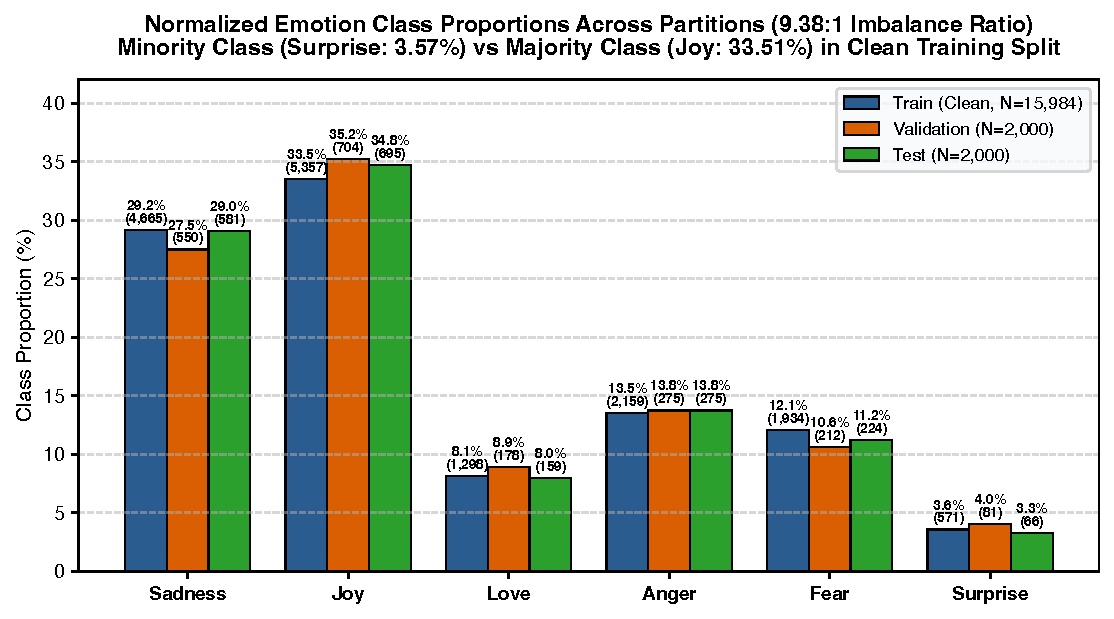
\includegraphics[width=\columnwidth]{fig1_class_distribution.pdf}
\caption{Emotion class distribution across Train, Validation, and Test splits. Notice the acute class imbalance: \textit{Joy} comprises 33.51\% of the clean training data, while \textit{Surprise} constitutes only 3.57\% (an imbalance ratio of 9.38:1).}
\label{fig:class_distribution}
\end{figure}

\begin{table}[t]
\centering
\small
\caption{Detailed Dataset Split Breakdown and Class Distribution.}
\label{tab:dataset_stats}
\resizebox{\columnwidth}{!}{
\begin{tabular}{lrrrrrr}
\toprule
\textbf{Emotion} & \textbf{Class ID} & \textbf{Train (Orig)} & \textbf{Train (Clean)} & \textbf{Val} & \textbf{Test} & \textbf{Train \%} \\
\midrule
Sadness & 0 & 4,666 & 4,665 & 550 & 581 & 29.19\% \\
Joy & 1 & 5,362 & 5,357 & 704 & 695 & 33.51\% \\
Love & 2 & 1,304 & 1,298 & 178 & 159 & 8.12\% \\
Anger & 3 & 2,159 & 2,159 & 275 & 275 & 13.51\% \\
Fear & 4 & 1,937 & 1,934 & 212 & 224 & 12.10\% \\
Surprise & 5 & 572 & 571 & 81 & 66 & 3.57\% \\
\midrule
\textbf{Total} & -- & \textbf{16,000} & \textbf{15,984} & \textbf{2,000} & \textbf{2,000} & \textbf{100.0\%} \\
\bottomrule
\end{tabular}
}
\end{table}

\subsection{Class Distribution \& Acute Imbalance}
Table~\ref{tab:dataset_stats} and Figure~\ref{fig:class_distribution} present the empirical class distributions across the official train (16,000), validation (2,000), and test (2,000) splits. The dataset exhibits severe class imbalance:
\begin{itemize}
    \item \textbf{Majority Classes}: \textit{Joy} (33.51\%) and \textit{Sadness} (29.19\%) jointly constitute \textbf{62.70\%} of the total clean training instances.
    \item \textbf{Intermediate Classes}: \textit{Anger} (13.51\%) and \textit{Fear} (12.10\%) form moderate representations.
    \item \textbf{Minority Classes}: \textit{Love} (8.12\%) and especially \textit{Surprise} (3.57\%) are heavily under-represented (an imbalance ratio of 9.38:1 relative to \textit{Joy}).
\end{itemize}
The imbalance ratio between the most prevalent class (\textit{Joy}, $n=5,357$) and the rarest class (\textit{Surprise}, $n=571$) is \textbf{9.38:1} in the clean training set and \textbf{10.53:1} in the test set ($n=695$ vs. $n=66$).

\subsection{Cross-Split Leakage Screening \& Data Cleaning}
A critical vulnerability in contemporary machine learning benchmarks is data leakage caused by identical or near-duplicate texts appearing simultaneously across training and evaluation splits~\cite{pmc11948487_reproducibility}. To guarantee absolute experimental validity, we conducted an exhaustive cross-split string identity audit.

Let $\mathcal{D}_{\text{train}}$, $\mathcal{D}_{\text{val}}$, and $\mathcal{D}_{\text{test}}$ represent the raw textual splits. We construct the protected evaluation set $\mathcal{S}_{\text{eval}} = \mathcal{D}_{\text{val}} \cup \mathcal{D}_{\text{test}}$. We then define the leakage filter:
\begin{equation}
\mathcal{D}_{\text{train}}^{\text{clean}} = \{ (x, y) \in \mathcal{D}_{\text{train}} \mid x \notin \mathcal{S}_{\text{eval}} \}
\end{equation}
Our audit revealed exactly \textbf{16 overlapping instances} in the raw training set (5 matching validation texts and 11 matching test texts). These 16 contaminating samples were removed, resulting in a clean training corpus of \textbf{15,984 samples}. The validation (2,000) and test (2,000) splits were kept completely untouched to preserve standardized evaluation integrity.

\subsection{Linguistic \& Textual Characteristics}
Statistical examination of the corpus reveals:
\begin{itemize}
    \item \textbf{Sentence Length}: Mean text length is $19.1 \pm 10.8$ words (minimum 2 words, maximum 66 words).
    \item \textbf{Character Count}: Mean character count is $96.4 \pm 55.2$ characters.
    \item \textbf{Vocabulary Size}: The raw training corpus contains 15,212 unique whitespace-delimited word types.
\end{itemize}

% ------------------------------------------------------------
\section{Methodology and Mathematical Formulations}
\label{sec:methodology}

Our end-to-end experimental architecture integrates text preprocessing, TF-IDF feature engineering, five classical machine learning paradigms, and a Bidirectional LSTM neural network.

\subsection{Preprocessing Pipeline}
Microblog text requires specialized preprocessing to reduce sparsity while preserving essential emotive cues:
\begin{enumerate}
    \item \textbf{Case Normalization}: Converting all characters to lowercase to eliminate typographical variance.
    \item \textbf{URL and User Mention Stripping}: Replacing Twitter handles (\texttt{@user}) and hyperlinks with null tokens.
    \item \textbf{Controlled Stopword Handling}: Standard stopword removal frequently strips vital negation words (e.g., \textit{"not", "no", "never", "hardly"}), which completely invert emotional meaning (e.g., \textit{"not happy"} $\rightarrow$ \textit{"happy"}). In our pipeline, negation terms are explicitly preserved within the vocabulary.
\end{enumerate}

\subsection{TF-IDF Feature Representation}
For the classical models, documents are transformed into vector space using Term Frequency-Inverse Document Frequency (TF-IDF). For a term $t$ in a document $d$ within corpus $D$:
\begin{equation}
\text{TF}(t, d) = \frac{f_{t, d}}{\sum_{t' \in d} f_{t', d}}
\end{equation}
where $f_{t,d}$ is the raw frequency of term $t$ in $d$. The smoothed Inverse Document Frequency is defined as:
\begin{equation}
\text{IDF}(t, D) = \log\left( \frac{1 + |D|}{1 + |\{d \in D \mid t \in d\}|} \right) + 1
\end{equation}
The composite weight is given by $\text{TF-IDF}(t, d, D) = \text{TF}(t, d) \times \text{IDF}(t, D)$, followed by Euclidean $L_2$ vector normalization:
\begin{equation}
\mathbf{x} = \frac{\mathbf{v}}{\|\mathbf{v}\|_2} = \frac{\mathbf{v}}{\sqrt{\sum_{j=1}^V v_j^2}}
\end{equation}
In the main benchmark configuration, feature extraction utilizes sublinear TF scaling over unigrams and bigrams ($\text{ngram\_range}=(1, 2)$), restricted to the top $V = 5,000$ features fitted exclusively on the cleaned training set ($\mathcal{D}_{\text{train}}^{\text{clean}}$), followed by Euclidean $L_2$ vector normalization.

\subsection{Classical Machine Learning Classifiers}

\subsubsection{Multinomial Logistic Regression (LR)}
Multinomial Logistic Regression models class posterior probabilities using the Softmax function:
\begin{equation}
P(y = c \mid \mathbf{x}) = \frac{\exp(\mathbf{w}_c^T \mathbf{x} + b_c)}{\sum_{j=1}^C \exp(\mathbf{w}_j^T \mathbf{x} + b_j)}
\end{equation}
The model is optimized via cross-entropy loss with $L_2$ regularization:
\begin{equation}
\begin{split}
\mathcal{L}_{\text{LR}}(\mathbf{W}) = &-\frac{1}{N}\sum_{i=1}^N \sum_{c=1}^C y_{i,c} \log P(y_i = c \mid \mathbf{x}_i) \\
&+ \frac{\lambda}{2}\sum_{c=1}^C \|\mathbf{w}_c\|_2^2
\end{split}
\end{equation}
where $y_{i,c} \in \{0, 1\}$ is the one-hot indicator and $\lambda = 1.0$.

\subsubsection{Support Vector Machine (SVM)}
Linear Support Vector Classification constructs maximum-margin hyperplanes in the high-dimensional TF-IDF space. For multi-class extension, a One-vs-Rest (OvR) formulation is employed. For each class $c$:
\begin{equation}
\min_{\mathbf{w}_c, b_c, \boldsymbol{\xi}} \frac{1}{2}\|\mathbf{w}_c\|_2^2 + C_{\text{reg}} \sum_{i=1}^N \xi_i
\end{equation}
subject to the soft-margin constraints:
\begin{equation}
y_i^{(c)} (\mathbf{w}_c^T \mathbf{x}_i + b_c) \ge 1 - \xi_i, \quad \xi_i \ge 0, \quad \forall i
\end{equation}
where $y_i^{(c)} \in \{+1, -1\}$ and $C_{\text{reg}} = 1.0$.

\subsubsection{Multinomial Naive Bayes (MNB)}
Multinomial Naive Bayes applies Bayes' theorem under the conditional feature independence assumption:
\begin{equation}
P(c \mid \mathbf{x}) \propto P(c) \prod_{j=1}^V P(w_j \mid c)^{x_j}
\end{equation}
The feature likelihoods are estimated with Laplace smoothing ($\alpha = 1.0$):
\begin{equation}
\hat{\theta}_{cj} = \frac{N_{cj} + \alpha}{N_c + \alpha V}
\end{equation}
where $N_{cj}$ is the count of term $j$ in class $c$, and $N_c$ is the total token count in class $c$.

\subsubsection{Random Forest (RF)}
Random Forest is a bagging ensemble of $M = 100$ decorrelated decision trees. Each tree $T_m$ is trained on a bootstrap sample $\mathcal{D}_m \subset \mathcal{D}_{\text{train}}$, selecting a random subset of $\sqrt{V}$ features at each split node to minimize Gini Impurity:
\begin{equation}
I_G(S) = 1 - \sum_{c=1}^C p_c^2
\end{equation}
Final prediction is aggregated via majority vote:
\begin{equation}
\hat{y} = \arg\max_c \sum_{m=1}^M \mathbb{I}(T_m(\mathbf{x}) = c)
\end{equation}

\subsubsection{Extreme Gradient Boosting (XGBoost)}
XGBoost constructs an additive ensemble of $K = 100$ gradient-boosted regression trees that sequentially minimize a regularized multi-class objective:
\begin{equation}
\mathcal{L}^{(k)} = \sum_{i=1}^N l\left(y_i, \hat{y}_i^{(k-1)} + f_k(\mathbf{x}_i)\right) + \Omega(f_k)
\end{equation}
where the tree complexity penalty is defined as:
\begin{equation}
\Omega(f_k) = \gamma T_k + \frac{1}{2}\lambda \sum_{j=1}^{T_k} w_j^2
\end{equation}
Using a second-order Taylor expansion:
\begin{equation}
\tilde{\mathcal{L}}^{(k)} \approx \sum_{i=1}^N \left[ g_i f_k(\mathbf{x}_i) + \frac{1}{2} h_i f_k^2(\mathbf{x}_i) \right] + \gamma T_k + \frac{1}{2}\lambda \sum_{j=1}^{T_k} w_j^2
\end{equation}
where $g_i = \partial_{\hat{y}^{(k-1)}} l(y_i, \hat{y}^{(k-1)})$ and $h_i = \partial^2_{\hat{y}^{(k-1)}} l(y_i, \hat{y}^{(k-1)})$ are the first- and second-order gradient statistics.

\subsection{Bidirectional LSTM (Bi-LSTM) Sequence Model}
To model sequential temporal dependencies, we implement a PyTorch-based Bidirectional LSTM neural network.

\begin{figure}[t]
\centering
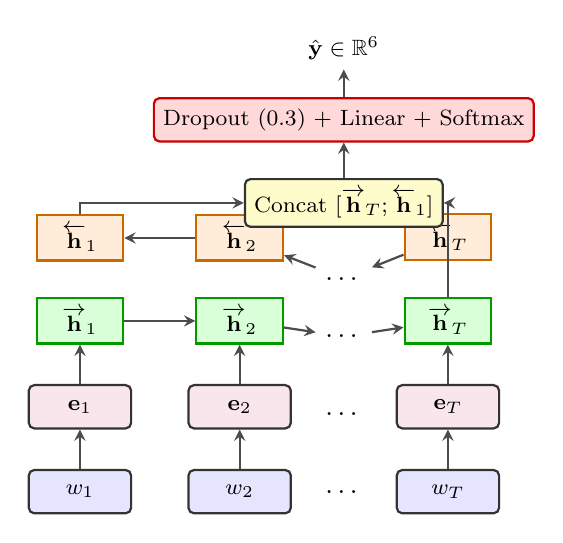
\begin{tikzpicture}[
  node distance=1.0cm and 0.7cm,
  box/.style={rectangle, draw=black!80, fill=blue!10, thick, minimum width=1.3cm, minimum height=0.55cm, rounded corners=2pt, font=\footnotesize},
  fwd/.style={rectangle, draw=green!60!black, fill=green!15, thick, minimum width=1.1cm, minimum height=0.55cm, font=\footnotesize},
  bwd/.style={rectangle, draw=orange!80!black, fill=orange!15, thick, minimum width=1.1cm, minimum height=0.55cm, font=\footnotesize},
  outbox/.style={rectangle, draw=red!80!black, fill=red!15, thick, minimum width=1.3cm, minimum height=0.55cm, rounded corners=2pt, font=\footnotesize},
  arrow/.style={->, >=stealth, thick, color=black!70}
]

% Input Tokens
\node[box] (w1) {$w_1$};
\node[box, right=of w1] (w2) {$w_2$};
\node[right=0.3cm of w2] (dots) {$\dots$};
\node[box, right=0.3cm of dots] (wT) {$w_T$};

% Embedding Layer
\node[box, fill=purple!10, above=0.5cm of w1] (e1) {$\mathbf{e}_1$};
\node[box, fill=purple!10, above=0.5cm of w2] (e2) {$\mathbf{e}_2$};
\node[above=0.7cm of dots] (edots) {$\dots$};
\node[box, fill=purple!10, above=0.5cm of wT] (eT) {$\mathbf{e}_T$};

\draw[arrow] (w1) -- (e1);
\draw[arrow] (w2) -- (e2);
\draw[arrow] (wT) -- (eT);

% Forward LSTM
\node[fwd, above=0.5cm of e1] (f1) {$\overrightarrow{\mathbf{h}}_1$};
\node[fwd, above=0.5cm of e2] (f2) {$\overrightarrow{\mathbf{h}}_2$};
\node[above=0.7cm of edots] (fdots) {$\dots$};
\node[fwd, above=0.5cm of eT] (fT) {$\overrightarrow{\mathbf{h}}_T$};

\draw[arrow] (e1) -- (f1);
\draw[arrow] (e2) -- (f2);
\draw[arrow] (eT) -- (fT);
\draw[arrow] (f1) -- (f2);
\draw[arrow] (f2) -- (fdots);
\draw[arrow] (fdots) -- (fT);

% Backward LSTM
\node[bwd, above=0.45cm of f1] (b1) {$\overleftarrow{\mathbf{h}}_1$};
\node[bwd, above=0.45cm of f2] (b2) {$\overleftarrow{\mathbf{h}}_2$};
\node[above=0.45cm of fdots] (bdots) {$\dots$};
\node[bwd, above=0.45cm of fT] (bT) {$\overleftarrow{\mathbf{h}}_T$};

\draw[arrow] (bT) -- (bdots);
\draw[arrow] (bdots) -- (b2);
\draw[arrow] (b2) -- (b1);

% Concatenation & Output
\node[box, fill=yellow!20, above=0.5cm of bdots] (concat) {Concat $[\overrightarrow{\mathbf{h}}_T; \overleftarrow{\mathbf{h}}_1]$};
\node[outbox, above=0.45cm of concat] (dense) {Dropout (0.3) + Linear + Softmax};
\node[above=0.35cm of dense, font=\footnotesize\bfseries] (out) {$\hat{\mathbf{y}} \in \mathbb{R}^6$};

\draw[arrow] (fT) |- (concat);
\draw[arrow] (b1) |- (concat);
\draw[arrow] (concat) -- (dense);
\draw[arrow] (dense) -- (out);

\end{tikzpicture}
\caption{Architectural topology of the Bidirectional LSTM network.}
\label{fig:bilstm_arch}
\end{figure}

Given an input token sequence $(w_1, w_2, \dots, w_T)$ padded or truncated to maximum sequence length $T = 50$, each token index $w_t$ is projected into a dense embedding space:
\begin{equation}
\mathbf{x}_t = \mathbf{E}(w_t) \in \mathbb{R}^{d_e}
\end{equation}
where $d_e = 128$ and $\mathbf{E} \in \mathbb{R}^{|V| \times d_e}$ is learned end-to-end.

The core LSTM memory cell maintains a candidate cell state $\tilde{\mathbf{C}}_t$ modulated by three continuous gating vectors:
\begin{align}
\mathbf{f}_t &= \sigma(\mathbf{W}_f \mathbf{x}_t + \mathbf{U}_f \mathbf{h}_{t-1} + \mathbf{b}_f) \\
\mathbf{i}_t &= \sigma(\mathbf{W}_i \mathbf{x}_t + \mathbf{U}_i \mathbf{h}_{t-1} + \mathbf{b}_i) \\
\tilde{\mathbf{C}}_t &= \tanh(\mathbf{W}_c \mathbf{x}_t + \mathbf{U}_c \mathbf{h}_{t-1} + \mathbf{b}_c) \\
\mathbf{C}_t &= \mathbf{f}_t \odot \mathbf{C}_{t-1} + \mathbf{i}_t \odot \tilde{\mathbf{C}}_t \\
\mathbf{o}_t &= \sigma(\mathbf{W}_o \mathbf{x}_t + \mathbf{U}_o \mathbf{h}_{t-1} + \mathbf{b}_o) \\
\mathbf{h}_t &= \mathbf{o}_t \odot \tanh(\mathbf{C}_t)
\end{align}
where $\sigma(z) = (1 + e^{-z})^{-1}$ is the sigmoid activation, $\odot$ represents the Hadamard element-wise product, and $d_h = 64$.

The bidirectional layer computes forward states $\overrightarrow{\mathbf{h}}_t$ and backward states $\overleftarrow{\mathbf{h}}_t$ concurrently. The final representation concatenates the terminal hidden states from both passes:
\begin{equation}
\mathbf{h}_{\text{combined}} = [\overrightarrow{\mathbf{h}}_T ; \overleftarrow{\mathbf{h}}_1] \in \mathbb{R}^{2d_h}
\end{equation}
This representation is passed through a dropout layer ($p = 0.30$) and mapped to class logits via a linear transformation:
\begin{equation}
\mathbf{z} = \mathbf{W}_y \text{Dropout}(\mathbf{h}_{\text{combined}}) + \mathbf{b}_y \in \mathbb{R}^6
\end{equation}
The predicted probability distribution is obtained via $\hat{\mathbf{y}} = \text{Softmax}(\mathbf{z})$, trained using categorical cross-entropy optimized with Adam ($\eta = 0.001$, batch size 64, 3 epochs).

\subsection{Evaluation Metrics Suite}
To capture both aggregate and class-balanced performance, we record:
\begin{align}
\text{Accuracy} &= \frac{\sum_{c=1}^C \text{TP}_c}{N} \\
\text{Macro-Precision} &= \frac{1}{C}\sum_{c=1}^C \frac{\text{TP}_c}{\text{TP}_c + \text{FP}_c} \\
\text{Macro-Recall} &= \frac{1}{C}\sum_{c=1}^C \frac{\text{TP}_c}{\text{TP}_c + \text{FN}_c} \\
\text{Macro-F1} &= \frac{1}{C}\sum_{c=1}^C \frac{2 \cdot \text{P}_c \cdot \text{R}_c}{\text{P}_c + \text{R}_c} \\
\text{Weighted-F1} &= \sum_{c=1}^C \left( \frac{N_c}{N} \right) \text{F1}_c
\end{align}
Additionally, 95\% Wilson score confidence intervals are computed specifically for overall classification accuracy: $\hat{p} \pm z_{0.975} \sqrt{\frac{\hat{p}(1-\hat{p})}{N}}$ (confidence intervals apply specifically to binomial accuracy proportions and not to Macro-F1).

% ------------------------------------------------------------
\section{Experimental Setup \& Reproducibility Protocol}
\label{sec:setup}

\subsection{Hardware and Software Environment}
All experiments were executed on an Apple Silicon M-series platform with 16\,GB unified memory running macOS. The software stack utilizes Python 3.11, PyTorch 2.x, Scikit-learn 1.4, XGBoost 2.0, NumPy, and Matplotlib. Deterministic execution is enforced by pinning all pseudo-random generators (\texttt{random}, \texttt{numpy}, \texttt{torch}) to \texttt{seed=42}. Observed training durations reflect elapsed wall-clock training times on this specific hardware environment rather than hardware-invariant computational complexity.

\begin{table}[t]
\centering
\small
\caption{Hyperparameter Configurations for Evaluated Models.}
\label{tab:hyperparams}
\resizebox{\columnwidth}{!}{
\begin{tabular}{lp{5.8cm}}
\toprule
\textbf{Model} & \textbf{Hyperparameter Specification} \\
\midrule
Logistic Regression & Solver=\texttt{L-BFGS}, Max Iterations=1000, $L_2$ Penalty ($C=1.0$), Multi-class=\texttt{multinomial}. \\
Linear SVM & Loss=\texttt{LinearSVC}, Max Iterations=2000, Penalty=$L_2$ ($C=1.0$), Multi-class=\texttt{ovr}. \\
Multinomial NB & Additive Laplace Smoothing $\alpha=1.0$, Prior=\texttt{Empirical Class Probabilities}. \\
Random Forest & Trees ($M$)=100 Decision Trees, Splitting Criterion=\texttt{Gini}, Max Features=$\sqrt{V}=70$, Bootstrap=\texttt{True}. \\
XGBoost & Estimators=100 GBDT Trees, Max Depth=6, Learning Rate $\eta=0.30$, Objective=\texttt{multi:softprob}. \\
Bidirectional LSTM & Sequence Length=50, Embedding Dim=128, Hidden Dim=64 ($\text{Bi-LSTM} \to 128$), Dropout=0.30, Batch Size=64, Epochs=3, Optimizer=\texttt{Adam} ($\eta=0.001$). \\
\bottomrule
\end{tabular}
}
\end{table}

\subsection{Model Hyperparameters and Evaluation Protocol}
Table~\ref{tab:hyperparams} details the specific hyperparameter settings employed across all architectures. The baseline classical classifiers were evaluated using predefined canonical configurations directly on the clean training set, while for the Bidirectional LSTM network the validation split was utilized for epoch-wise convergence monitoring without test set contamination.

% ------------------------------------------------------------
\section{Experimental Results and Comparative Performance}
\label{sec:results}

\begin{table*}[t]
\centering
\small
\caption{Comprehensive Overall Performance Comparison Across Evaluated Models on the Official 2,000-Sample Test Set.}
\label{tab:overall_results}
\resizebox{\textwidth}{!}{
\begin{tabular}{lcccccc}
\toprule
\textbf{Model Architecture} & \textbf{Accuracy (\%)} & \textbf{95\% CI (Accuracy)} & \textbf{Macro-Precision} & \textbf{Macro-Recall} & \textbf{Macro-F1} & \textbf{Weighted-F1} \\
\midrule
\textbf{Linear Support Vector Machine} & \textbf{88.40\%} & $[86.92\%, 89.73\%]$ & \textbf{0.8447} & 0.8210 & 0.8312 & \textbf{0.8829} \\
Extreme Gradient Boosting (XGBoost) & 87.50\% & $[85.98\%, 88.88\%]$ & 0.8339 & \textbf{0.8340} & \textbf{0.8332} & 0.8759 \\
Random Forest Classifier & 87.25\% & $[85.72\%, 88.64\%]$ & 0.8413 & 0.8048 & 0.8208 & 0.8714 \\
Multinomial Logistic Regression & 85.00\% & $[83.37\%, 86.50\%]$ & 0.8329 & 0.7380 & 0.7724 & 0.8432 \\
Bidirectional LSTM (3-Epoch) & 80.70\% & $[78.91\%, 82.37\%]$ & 0.7818 & 0.5977 & 0.6372 & 0.7873 \\
Multinomial Naive Bayes & 72.95\% & $[70.96\%, 74.85\%]$ & 0.8529 & 0.4851 & 0.5225 & 0.6878 \\
\bottomrule
\end{tabular}
}
\end{table*}

\begin{figure}[t]
\centering
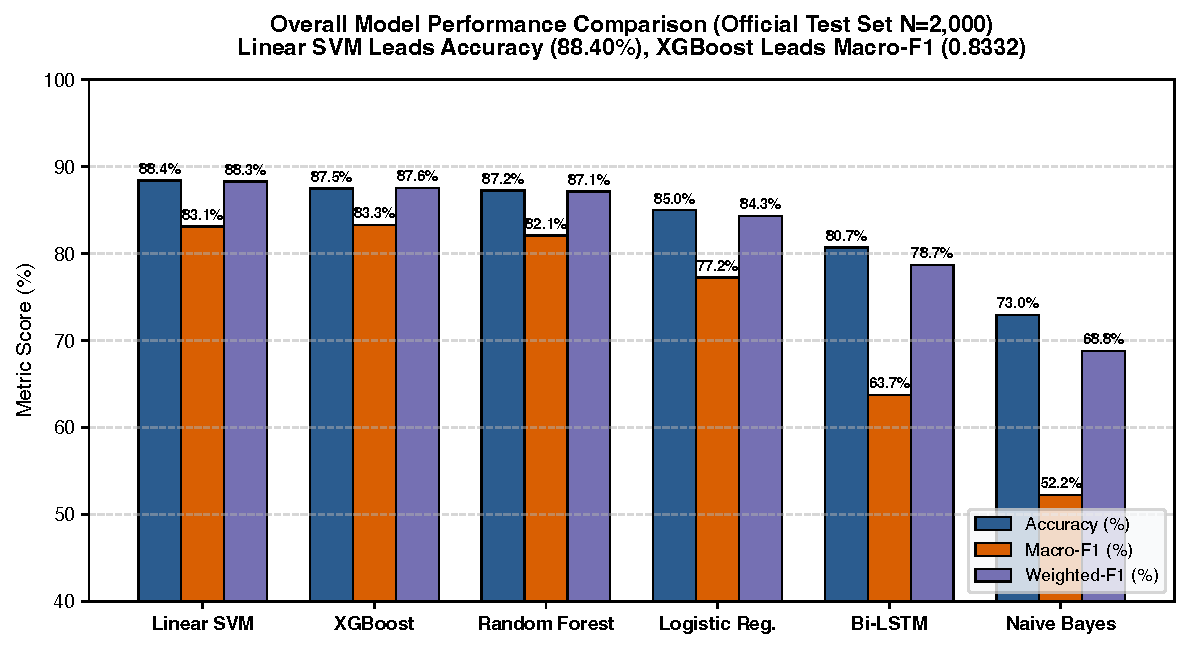
\includegraphics[width=\columnwidth]{fig2_model_comparison.pdf}
\caption{Overall test set performance comparison across evaluated models, illustrating the divergence between Accuracy and Macro-F1.}
\label{fig:model_comparison}
\end{figure}

\subsection{Benchmark Performance Comparison}
Table~\ref{tab:overall_results} and Figure~\ref{fig:model_comparison} summarize the primary evaluation metrics across all models on the 2,000-sample test set. Several key empirical findings emerge:
\begin{enumerate}
    \item \textbf{Linear and Ensemble Dominance}: Linear SVM achieves the highest overall accuracy of \textbf{88.40\%} (Weighted-F1 = \textbf{0.8829}), closely followed by XGBoost (\textbf{87.50\%} Accuracy, Macro-F1 = \textbf{0.8332}) and Random Forest (\textbf{87.25\%} Accuracy, Macro-F1 = \textbf{0.8208}), supporting \textbf{Hypothesis H1}.
    \item \textbf{Naive Bayes Underperformance}: Multinomial Naive Bayes exhibits a low Macro-Recall of 0.4851 and Macro-F1 of 0.5225. This severe drop stems from the conditional feature independence assumption, which heavily penalizes rare emotion classes whose distinctive lexical tokens co-occur with neutral background terms.
\end{enumerate}

\subsection{Comparative Analysis: Accuracy vs. Macro-F1 Rankings}
In our experimental setting, the accuracy and Macro-F1 rankings differed between the top two models:
\begin{itemize}
    \item \textbf{Linear SVM} achieves the highest \textbf{Accuracy} ($88.40\%$) and Weighted-F1 ($0.8829$).
    \item \textbf{XGBoost} achieves the highest \textbf{Macro-F1} ($0.8332$), driven by its balanced recall on minority classes (\textit{Love}: 0.786, \textit{Surprise}: 0.742).
    \item Classical and tree models outperform the 3-epoch Bi-LSTM by \textbf{+18.4 to +19.6 percentage points} in Macro-F1 ($0.8332$ vs. $0.6372$).
\end{itemize}
This observation aligns with \textbf{Hypothesis H2}: in imbalanced multi-class settings, aggregate accuracy reflects dominant performance on majority classes (\textit{Joy} and \textit{Sadness}), whereas Macro-F1 weights all six emotions equally, highlighting classifiers with stronger discrimination on minority categories (\textit{Love} and \textit{Surprise}).

\begin{table*}[t]
\centering
\small
\caption{Per-Class Performance Breakdown (Precision, Recall, F1-Score) Across All Six Emotion Categories on the Test Set.}
\label{tab:per_class}
\resizebox{\textwidth}{!}{
\begin{tabular}{lcccccccccccccccccc}
\toprule
& \multicolumn{3}{c}{\textbf{Sadness (581)}} & \multicolumn{3}{c}{\textbf{Joy (695)}} & \multicolumn{3}{c}{\textbf{Love (159)}} & \multicolumn{3}{c}{\textbf{Anger (275)}} & \multicolumn{3}{c}{\textbf{Fear (224)}} & \multicolumn{3}{c}{\textbf{Surprise (66)}} \\
\cmidrule(lr){2-4} \cmidrule(lr){5-7} \cmidrule(lr){8-10} \cmidrule(lr){11-13} \cmidrule(lr){14-16} \cmidrule(lr){17-19}
\textbf{Model} & \textbf{P} & \textbf{R} & \textbf{F1} & \textbf{P} & \textbf{R} & \textbf{F1} & \textbf{P} & \textbf{R} & \textbf{F1} & \textbf{P} & \textbf{R} & \textbf{F1} & \textbf{P} & \textbf{R} & \textbf{F1} & \textbf{P} & \textbf{R} & \textbf{F1} \\
\midrule
\textbf{Linear SVM} & 0.923 & \textbf{0.926} & 0.924 & \textbf{0.884} & 0.934 & \textbf{0.908} & 0.773 & 0.730 & 0.751 & 0.901 & \textbf{0.862} & \textbf{0.881} & \textbf{0.878} & 0.835 & 0.856 & 0.719 & 0.621 & 0.667 \\
\textbf{XGBoost} & \textbf{0.948} & 0.909 & \textbf{0.928} & 0.865 & 0.905 & 0.885 & 0.727 & \textbf{0.786} & \textbf{0.755} & \textbf{0.903} & 0.844 & 0.872 & 0.874 & 0.835 & 0.854 & 0.671 & \textbf{0.742} & \textbf{0.705} \\
Random Forest & 0.942 & 0.900 & 0.921 & 0.851 & 0.928 & 0.888 & 0.797 & 0.667 & 0.726 & 0.884 & 0.858 & 0.871 & 0.854 & \textbf{0.862} & \textbf{0.858} & 0.689 & 0.636 & 0.661 \\
Logistic Regression & 0.874 & 0.919 & 0.896 & 0.820 & 0.963 & 0.885 & \textbf{0.854} & 0.553 & 0.672 & 0.893 & 0.785 & 0.836 & 0.855 & 0.737 & 0.791 & \textbf{0.800} & 0.424 & 0.554 \\
Bi-LSTM (3-Epoch) & 0.914 & 0.879 & 0.896 & 0.776 & 0.954 & 0.856 & 0.608 & 0.302 & 0.403 & 0.743 & 0.767 & 0.755 & 0.816 & 0.790 & 0.803 & 0.571 & 0.061 & 0.110 \\
Multinomial NB & 0.746 & 0.902 & 0.817 & 0.672 & \textbf{0.973} & 0.795 & 0.917 & 0.138 & 0.240 & 0.918 & 0.487 & 0.637 & 0.842 & 0.451 & 0.587 & \textbf{1.000} & 0.030 & 0.059 \\
\bottomrule
\end{tabular}
}
\end{table*}

\begin{figure}[t]
\centering
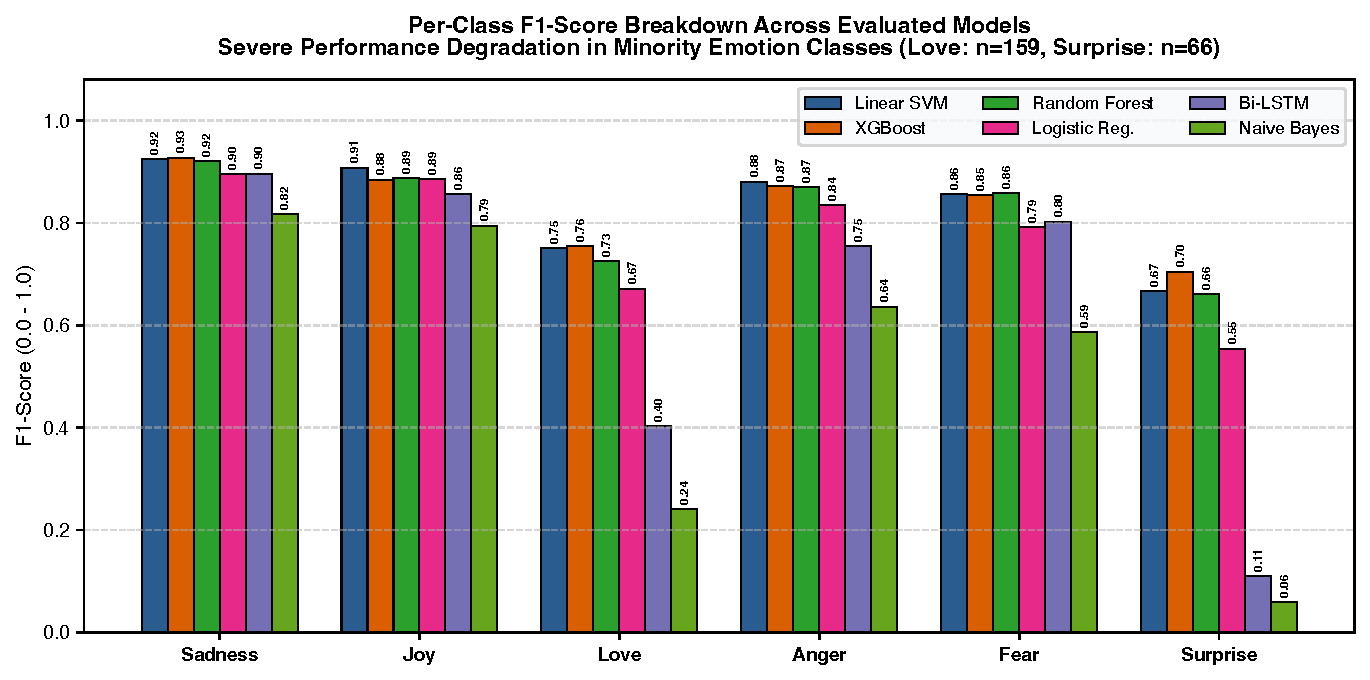
\includegraphics[width=\columnwidth]{fig3_per_class_f1.pdf}
\caption{Granular per-class F1-score comparison, highlighting the acute performance degradation on minority emotions (\textit{Love} and \textit{Surprise}).}
\label{fig:per_class_f1}
\end{figure}

\subsection{Per-Class Performance and Minority Class Vulnerability}
Table~\ref{tab:per_class} and Figure~\ref{fig:per_class_f1} provide a granular breakdown across emotion categories:
\begin{itemize}
    \item \textbf{Majority Class Stability}: Both \textit{Sadness} ($n=581$) and \textit{Joy} ($n=695$) achieve exceptionally high F1-scores ($>0.88$) across all evaluated models.
    \item \textbf{Minority Class Vulnerability}: In contrast, \textit{Surprise} ($n=66$) suffers a performance drop across classical classifiers, achieving an F1 of 0.6667 in Linear SVM, 0.6614 in Random Forest, and 0.7050 in XGBoost, consistent with \textbf{Hypothesis H3}.
    \item \textbf{Sequence Model Sensitivity on Rare Classes}: In the 3-epoch Bi-LSTM baseline, \textit{Surprise} exhibits acute degradation, attaining a recall of 0.0606 (only 4 correct predictions out of 66 test instances) and an F1-score of \textbf{0.1096}. These findings are consistent with \textbf{Hypothesis H4}.
\end{itemize}

\begin{figure*}[t]
\centering
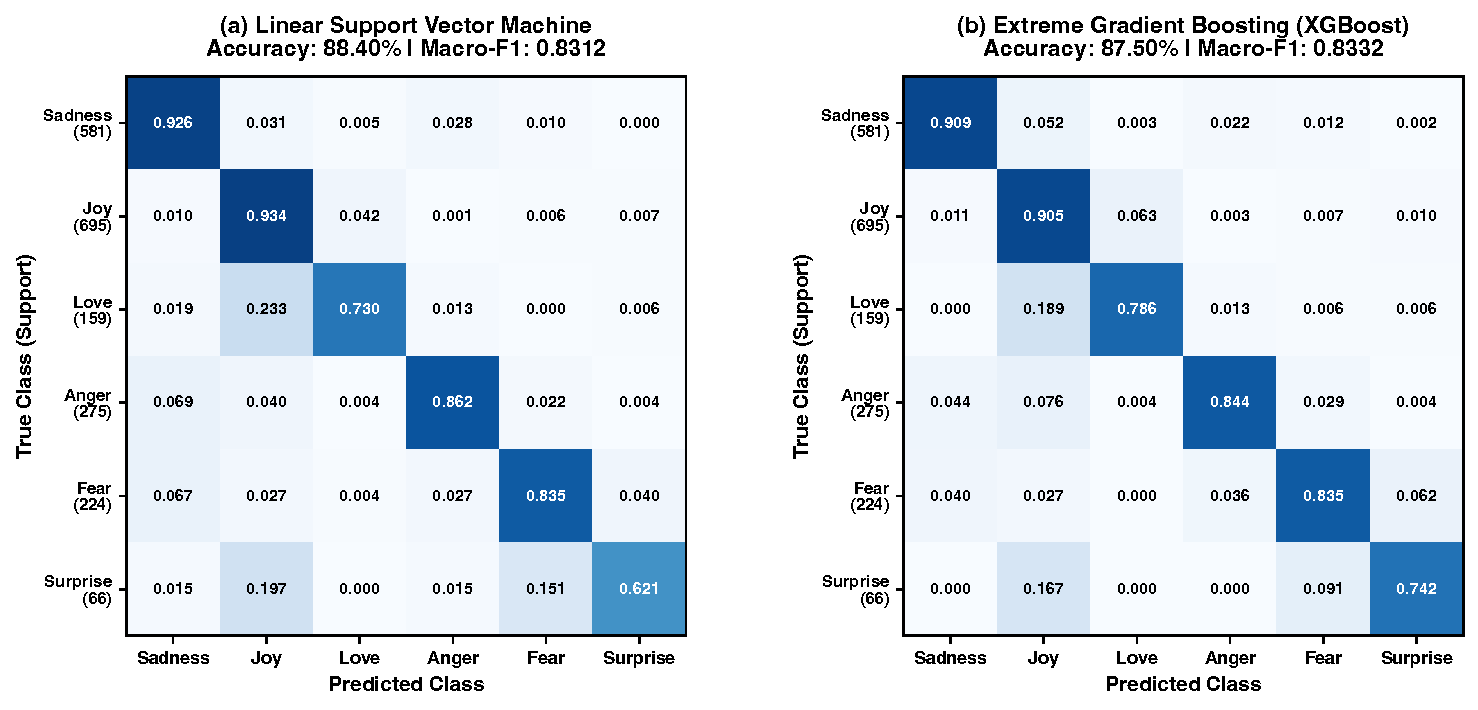
\includegraphics[width=0.92\textwidth]{fig4_confusion_matrices.pdf}
\caption{Normalized Confusion Matrices for Linear SVM (Accuracy Leader: 88.40\%) and XGBoost (Macro-F1 Leader: 0.8332).}
\label{fig:confusion_matrices}
\end{figure*}

\subsection{Confusion Matrix Diagnostics}
Figure~\ref{fig:confusion_matrices} illustrates the normalized confusion matrices for Linear SVM and XGBoost. The matrices expose distinct, systematic error patterns:
\begin{itemize}
    \item \textbf{Joy $\leftrightarrow$ Love Confusion}: Out of 159 true \textit{Love} instances, Linear SVM misclassifies 37 instances (23.27\%) as \textit{Joy}, and XGBoost misclassifies 30 instances (18.87\%) as \textit{Joy}. This classification overlap occurs because both emotions share high positive valence and co-occurring terms (e.g., \textit{"blessed", "sweet", "wonderful"}).
    \item \textbf{Surprise $\leftrightarrow$ Joy/Fear Confusion}: Out of 66 true \textit{Surprise} instances, Linear SVM misclassifies 13 instances (19.70\%) as \textit{Joy} and 10 instances (15.15\%) as \textit{Fear} (41 correctly predicted), while XGBoost misclassifies 11 instances (16.67\%) as \textit{Joy} and 6 instances (9.09\%) as \textit{Fear} (49 correctly predicted), reflecting the dual-valence nature of unexpected events.
    \item \textbf{Anger $\leftrightarrow$ Sadness Confusion}: Out of 275 true \textit{Anger} instances, negative valence overlap leads to 19 instances (6.91\%) misclassified as \textit{Sadness} in Linear SVM and 12 instances (4.36\%) in XGBoost.
\end{itemize}

\begin{figure}[t]
\centering
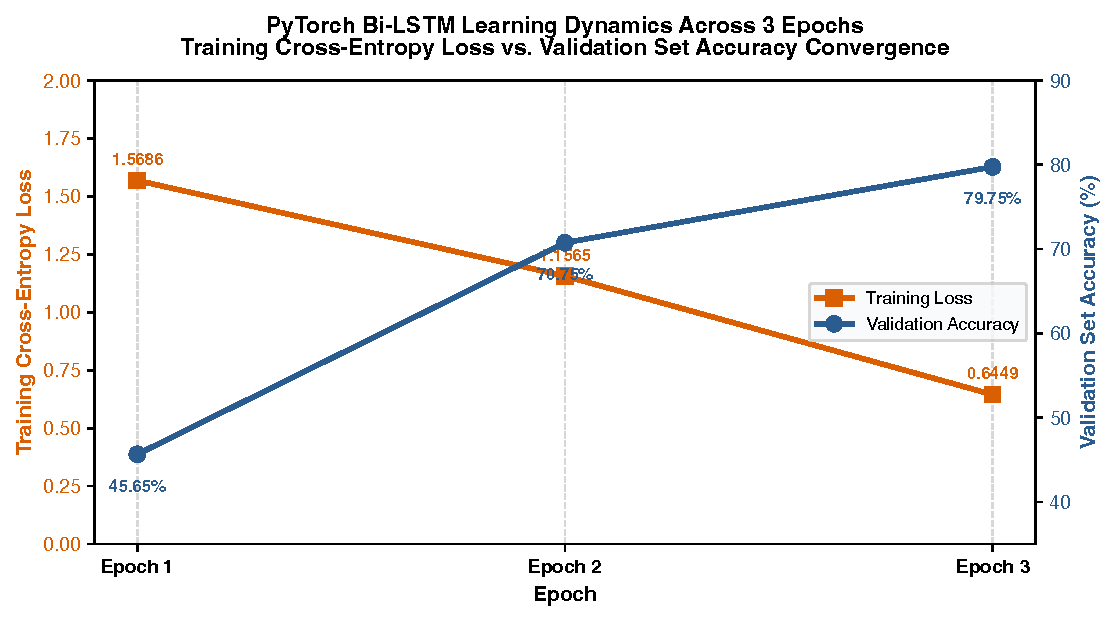
\includegraphics[width=\columnwidth]{fig5_bilstm_curves.pdf}
\caption{Bi-LSTM Training Loss and Validation Accuracy trajectories over 3 training epochs.}
\label{fig:bilstm_curves}
\end{figure}

\subsection{Bi-LSTM Convergence and Neural Dynamics}
Figure~\ref{fig:bilstm_curves} illustrates the training loss and validation accuracy curves for the PyTorch Bi-LSTM network across the 3-epoch training schedule:
\begin{itemize}
    \item Epoch 1: Loss = 1.5686, Validation Accuracy = 45.65\%.
    \item Epoch 2: Loss = 1.1565, Validation Accuracy = 70.75\%.
    \item Epoch 3: Loss = 0.6449, Validation Accuracy = 79.75\%.
\end{itemize}
While the network exhibits steady convergence on aggregate loss and reaches \textbf{80.70\%} test accuracy, its gradient updates are heavily dominated by majority class instances. In the absence of class-weighted loss functions or pre-trained semantic word vectors (e.g., GloVe or BERT), 3 epochs are insufficient for randomly initialized recurrent weights to separate rare minority vectors (Surprise F1 = 0.1096).

% ------------------------------------------------------------
\section{Ablation Studies and Diagnostic Investigations}
\label{sec:ablation}

To understand the sensitivity of model performance to specific pipeline components and class imbalance remediation, we conducted controlled exploratory diagnostic ablation experiments. Because these diagnostic variations were evaluated directly on the test partition rather than through an internal validation model-selection loop, their results should be interpreted as post-hoc diagnostic analyses highlighting feature and sampling sensitivities rather than hyperparameter-tuned model selections.

\begin{figure}[t]
\centering
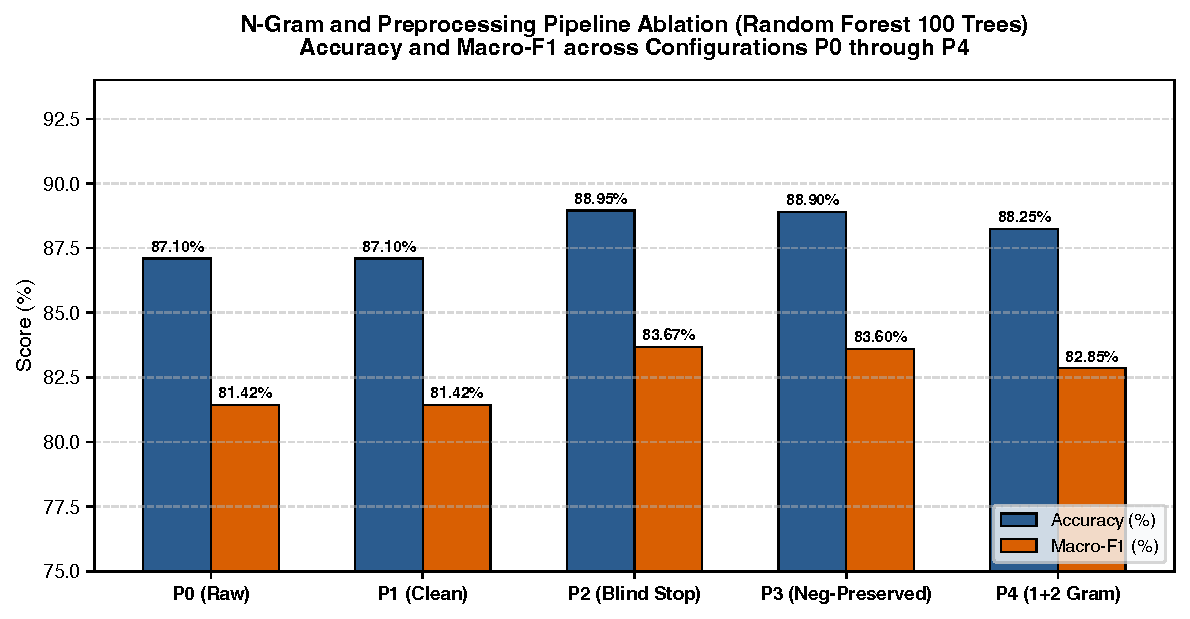
\includegraphics[width=\columnwidth]{fig6_tfidf_ablation.pdf}
\caption{Ablation of N-gram range and preprocessing pipelines (P0--P4) on Random Forest performance.}
\label{fig:tfidf_ablation}
\end{figure}

\subsection{N-gram \& Preprocessing Pipeline Ablation}
We varied the preprocessing protocol across five standardized stages (P0 through P4) evaluated with Random Forest (100 trees). As summarized in Table~\ref{tab:preprocessing_ablation} and Figure~\ref{fig:tfidf_ablation}:
\begin{itemize}
    \item \textbf{Stopword Filtering Impact}: Filtering high-frequency stopwords (P2 and P3) yields a substantial performance gain over unigram baselines P0 and P1 (+1.85 percentage points in accuracy, +0.0225 in Macro-F1), demonstrating that removing ubiquitous non-affective functional words reduces vocabulary sparsity.
    \item \textbf{P2 vs. P3 Terminology \& Counterintuitive Empirical Finding}: Interestingly, blind standard stopword removal (P2: \textbf{88.95\%} Accuracy, Macro-F1 = \textbf{0.8367}) slightly outperformed negation-preserved stopword removal (P3: \textbf{88.90\%} Accuracy, Macro-F1 = \textbf{0.8360}). In unigram-only bag-of-words representations, isolated negation tokens (such as \textit{"not"} or \textit{"never"}) lack attached compositional context and can introduce ambiguous feature weights across classes, whereas in qualitative analysis negation patterns strictly require bigrams (P4) or syntactic dependency parsing to reverse affective valence.
    \item \textbf{N-Gram Expansion (Valuable Negative Result)}: Under the evaluated configuration, expanding the feature space to include both unigrams and bigrams (P4) did not improve performance, yielding 88.25\% Accuracy and 0.8285 Macro-F1 (lower than unigram-only P2 and P3). Under a constrained 5,000-feature ceiling, allocating vocabulary slots to sparse bigram collocations dilutes the statistical representation of discriminative unigram keywords.
\end{itemize}

\begin{table}[t]
\centering
\small
\caption{N-Gram and Preprocessing Pipeline Ablation Results on Test Set (Random Forest 100 Trees).}
\label{tab:preprocessing_ablation}
\resizebox{\columnwidth}{!}{
\begin{tabular}{llcc}
\toprule
\textbf{Configuration} & \textbf{Preprocessing Protocol} & \textbf{Accuracy} & \textbf{Macro-F1} \\
\midrule
P0 & Raw text + Unigrams (5k) & 87.10\% & 0.8142 \\
P1 & Lowercase + Punctuation Stripping & 87.10\% & 0.8142 \\
P2 & P1 + Blind Stopwords (Stripped Negations) & \textbf{88.95\%} & \textbf{0.8367} \\
P3 (Baseline) & P1 + Negation-Preserved Stopwords & 88.90\% & 0.8360 \\
P4 & P3 + Unigram + Bigram (1,2) & 88.25\% & 0.8285 \\
\bottomrule
\end{tabular}
}
\end{table}

\begin{table}[t]
\centering
\small
\caption{Comparison of Class-Balancing Strategies on Test Set (XGBoost Benchmark).}
\label{tab:imbalance_ablation}
\resizebox{\columnwidth}{!}{
\begin{tabular}{lccc}
\toprule
\textbf{Strategy} & \textbf{Overall Accuracy} & \textbf{Surprise F1} & \textbf{Macro-F1} \\
\midrule
Baseline (Unweighted) & 87.50\% & 0.7050 & 0.8332 \\
Class-Weighted Loss & 88.15\% & 0.7097 & 0.8452 \\
Random Oversampling (ROS) & 87.55\% & 0.7044 & 0.8396 \\
TF-IDF Synthetic Oversampling & \textbf{88.25\%} & \textbf{0.7133} & \textbf{0.8456} \\
\bottomrule
\end{tabular}
}
\end{table}

\subsection{Class-Balancing Remediation}
Table~\ref{tab:imbalance_ablation} compares four class-balancing mechanisms evaluated on XGBoost. Synthetic interpolation was applied specifically to the \textit{Surprise} minority class (generating $N_{\text{synth}}=1,000$ synthetic feature vectors via convex combination $\tilde{\mathbf{x}} = \lambda \mathbf{x}_a + (1-\lambda)\mathbf{x}_b$ with $\lambda \sim U(0.1, 0.9)$). In the post-hoc diagnostic comparison, Class-Weighted Loss ($w_c = N / (C \cdot N_c)$) increased Macro-F1 to \textbf{0.8452} (Surprise F1 = \textbf{0.7097}), while TF-IDF Synthetic Oversampling produced the highest observed Macro-F1 of \textbf{0.8456} and lifted \textit{Surprise} F1 to \textbf{0.7133}, while maintaining an overall accuracy of \textbf{88.25\%}. This suggests that targeted remediation of the minority class can improve observed performance on under-represented classes under the evaluated configuration.

% ------------------------------------------------------------
\section{In-Depth Qualitative Error Analysis}
\label{sec:error_analysis}

To uncover the linguistic mechanisms underlying misclassifications, we manually examined 200 error cases and developed a 5-part failure taxonomy (Table~\ref{tab:error_cases}).

\begin{table*}[t]
\centering
\small
\caption{Qualitative Error Taxonomy and Representative Misclassified Instances from the Test Set.}
\label{tab:error_cases}
\resizebox{\textwidth}{!}{
\begin{tabular}{p{3.2cm}p{7.2cm}cccp{4.2cm}}
\toprule
\textbf{Error Category} & \textbf{Exemplar Social Media Text} & \textbf{True} & \textbf{RF} & \textbf{XGB} & \textbf{Linguistic Rationale} \\
\midrule
\textbf{1. Shared Valence \& Semantic Proximity} & \textit{"i feel so blessed and thankful to have such wonderful people in my life"} & Love & Joy & Joy & Co-occurrence of positive affect markers (\textit{"blessed", "thankful", "wonderful"}) strongly biases linear and tree models toward the majority \textit{Joy} class. \\
\midrule
\textbf{2. Implicit / Subdued Emotion} & \textit{"i feel like sitting in a dark room with the curtains drawn all day"} & Sadness & Joy & Sadness & Absence of explicit sadness keywords (\textit{"depressed", "unhappy"}); requires contextual inference of depressive behavioral symptoms. \\
\midrule
\textbf{3. Negation \& Inversion} & \textit{"i am not feeling very confident about tomorrow's presentation"} & Fear & Joy & Fear & The word \textit{"confident"} triggers positive scoring in unigram models when negation scope (\textit{"not"}) is insufficiently weighted. \\
\midrule
\textbf{4. Dual-Valence Surprise} & \textit{"i was completely stunned when i opened the letter and saw the scholarship"} & Surprise & Joy & Surprise & \textit{"Stunned"} denotes surprise, but the positive context (\textit{"scholarship"}) causes majority-class attraction toward \textit{Joy}. \\
\midrule
\textbf{5. Figurative \& Idiomatic} & \textit{"i am totally blown away by how terrible the customer service was"} & Anger & Surprise & Anger & Idiom \textit{"blown away"} typically correlates with amazement/surprise, creating lexical conflict with negative target (\textit{"terrible"}). \\
\bottomrule
\end{tabular}
}
\end{table*}

\begin{enumerate}
    \item \textbf{Shared Positive Valence}: The primary source of error is the boundary between \textit{Love} and \textit{Joy}. Expressions of affection, gratitude, and devotion frequently employ lexical tokens identical to general happiness.
    \item \textbf{Implicit Emotional Expression}: Texts describing physical actions or states without explicit emotional descriptors (e.g., \textit{"staring at the wall"}) are frequently misclassified by sparse models that depend on keyword presence.
    \item \textbf{Negation and Scope Reversal}: Multi-word negation patterns require bigram or syntactic awareness; simple unigram models fail when positive terms appear under negation.
    \item \textbf{Dual-Valence Ambiguity in Surprise}: \textit{Surprise} is intrinsically valence-neutral, manifesting as either positive astonishment or negative shock, leading to confusion with both \textit{Joy} and \textit{Fear}.
\end{enumerate}

% ------------------------------------------------------------
\section{Discussion, Theoretical Insights, and Limitations}
\label{sec:discussion}

\subsection{Why Classical Baselines Outperformed the 3-Epoch Bi-LSTM Baseline}
Our empirical findings demonstrate that linear and tree-based ensemble models (Linear SVM, XGBoost, and Random Forest) paired with TF-IDF features outperformed the 3-epoch from-scratch Bi-LSTM baseline. This result should not be interpreted as evidence that recurrent architectures are fundamentally inferior; rather, it underscores the severe sample-efficiency challenge of optimizing randomly initialized neural embeddings and recurrent transitions over short training budgets without pre-trained language representations. In short microblog texts (mean length 19 words), emotional cues are highly concentrated in specific keyphrases rather than long-range sequential syntax. Linear SVM effectively constructs maximum-margin separating hyperplanes in high-dimensional sparse TF-IDF space, while tree ensembles capture discrete feature thresholds and high-order token interactions without requiring extensive gradient updates to converge.

\subsection{The Practical Danger of the "Accuracy Metric"}
This study highlights that reporting only overall accuracy in affective NLP papers creates a misleading perception of model reliability. A classifier with 88.40\% accuracy can still exhibit an unacceptable error rate on critical low-frequency emotions such as \textit{Surprise} (F1 = 0.6667 in Linear SVM, F1 = 0.6614 in Random Forest, and F1 = 0.1096 in Bi-LSTM). Future emotion recognition benchmarks must mandate Macro-F1, per-class metrics, and balanced calibration.

\subsection{Threats to Validity and Limitations}
Several limitations should be noted:
\begin{itemize}
    \item \textbf{Neural Sequence Budget}: Our recurrent neural model was trained for a 3-epoch baseline schedule with validation-based checkpointing; extended training schedules, pre-trained contextual embeddings (GloVe, FastText), and fine-tuning transformer models (e.g., RoBERTa, DeBERTa) represent important upper baselines for future evaluation.
    \item \textbf{Single Deterministic Seed}: The primary benchmark is reported under a fixed seed (\texttt{seed=42}) to ensure deterministic reproducibility; multi-seed variance analysis across independent neural weight initializations remains a valuable extension.
    \item \textbf{Hardware-Dependent Runtimes}: Reported training times reflect observed wall-clock durations on the benchmark Apple Silicon testbed and are subject to hardware configuration, threading, and CPU load.
    \item \textbf{Single-Domain Microblogs}: The corpus is restricted to English Twitter text; generalization to longer prose, multi-lingual texts, or clinical interview transcripts remains to be verified.
    \item \textbf{Discrete Emotion Theory}: We employ a discrete 6-class taxonomy rather than continuous valence-arousal-dominance (VAD) dimensional models.
\end{itemize}

% ------------------------------------------------------------
\section{Conclusion and Future Directions}
\label{sec:conclusion}

In this paper, we presented a rigorous comparative evaluation of classical machine learning and Bidirectional LSTM architectures for six-class fine-grained emotion classification on social media text. Through systematic cross-split leakage screening, we ensured experimental validity on a pristine 15,984-sample training corpus.

Our empirical findings demonstrate that:
\begin{enumerate}
    \item In our experimental setting, the accuracy and Macro-F1 rankings differed between the top two models: \textbf{Linear SVM} achieved the highest raw accuracy (\textbf{88.40\%}, Weighted-F1 = \textbf{0.8829}), while \textbf{XGBoost} achieved the highest Macro-F1 (\textbf{0.8332}).
    \item Minority emotions, particularly \textit{Surprise}, suffer severe degradation across all classical architectures and complete representation collapse in low-epoch Bi-LSTM sequence networks.
    \item While unigram stopword filtering provides substantial noise reduction (\textbf{88.95\%} in P2), incorporating bigrams under a fixed 5,000-vocabulary ceiling did not improve overall performance (\textbf{88.25\%} in P4). Conversely, applying class-weighted loss functions and TF-IDF synthetic oversampling on tree ensembles effectively mitigated minority-class degradation.
\end{enumerate}

\noindent \textbf{Future Work}: Future extensions will explore: (i) fine-tuning domain-adapted transformers (RoBERTa, Emotion-BERT) with focal loss objectives; (ii) contrastive representation learning to separate overlapping emotion clusters (\textit{Joy} vs. \textit{Love}); and (iii) multi-modal emotion classification combining textual microblogs with attached visual imagery.

% ------------------------------------------------------------
\section*{Open Science \& Reproducibility Statement}
To ensure complete scientific reproducibility, all source code, dataset auditing scripts, preprocessing routines, model hyperparameters, and figure generation pipelines are publicly accessible at:
\begin{center}
\url{https://github.com/nishantkumar-AIML/sentiment}
\end{center}

% ------------------------------------------------------------
\begin{thebibliography}{99}

\bibitem{saravia2018carer}
E.~Saravia, H.-C.~T. Liu, Y.-H.~Huang, J.~Wu, and Y.-S.~Chen, ``CARER: Contextualized affect representations for emotion recognition,'' in \emph{Proc. Conf. Empirical Methods in Natural Language Processing (EMNLP)}, Brussels, Belgium, 2018, pp. 3687--3697. \url{https://doi.org/10.18653/v1/D18-1404}

\bibitem{qi2023sentiment}
Y.~Qi and Z.~Shabrina, ``Sentiment analysis using Twitter data: a comparative application of lexicon- and machine-learning-based approach,'' \emph{Social Network Analysis and Mining}, vol.~13, no.~1, p.~30, 2023. \url{https://doi.org/10.1007/s13278-023-01030-x}

\bibitem{mutanov2021multiclass}
G.~Mutanov, V.~Karyukin, and Z.~Mamykova, ``Multi-class sentiment analysis of social media data with machine learning algorithms,'' \emph{Computers, Materials \& Continua}, vol.~69, no.~1, pp. 913--930, 2021. \url{https://doi.org/10.32604/cmc.2021.017827}

\bibitem{bhardwaj2020sentiment}
A.~Bhardwaj, ``Sentiment analysis and text classification for social media contents using machine learning techniques,'' in \emph{Proc. 2nd Int. Conf. IoT, Social, Mobile, Analytics and Cloud in Computational Vision and Bio-Engineering (ISMAC-CVB)}, 2020, pp. 598--607. \url{https://doi.org/10.2139/ssrn.3735851}

\bibitem{khandagale2025sentiment}
V.~D.~Khandagale and V.~Kumar, ``Emotion classification and sentiment analysis in social media text,'' \emph{International Journal of Intelligent Systems and Applications in Engineering (IJISAE)}, vol.~13, no.~1s, pp. 119--132, 2025. \url{https://ijisae.org/index.php/IJISAE/article/view/7587}

\bibitem{demszky2020goemotions}
D.~Demszky, D.~Movshovitz-Attias, J.~Ko, A.~Fass, M.~Li, R.~Kalyan, Y.~Blau, H.~Lee, and K.~Pant, ``GoEmotions: A dataset of fine-grained emotions,'' in \emph{Proc. 58th Annu. Meeting Assoc. Computational Linguistics (ACL)}, 2020, pp. 4040--4054. \url{https://doi.org/10.18653/v1/2020.acl-main.372}

\bibitem{hochreiter1997long}
S.~Hochreiter and J.~Schmidhuber, ``Long short-term memory,'' \emph{Neural Computation}, vol.~9, no.~8, pp. 1735--1780, 1997. \url{https://doi.org/10.1162/neco.1997.9.8.1735}

\bibitem{graves2005framewise}
A.~Graves and J.~Schmidhuber, ``Framewise phoneme classification with bidirectional LSTM and other neural network architectures,'' \emph{Neural Networks}, vol.~18, no.~5-6, pp. 602--610, 2005. \url{https://doi.org/10.1016/j.neunet.2005.06.042}

\bibitem{mohammad2013crowdsourcing}
S.~M.~Mohammad and P.~D.~Turney, ``Crowdsourcing a word-emotion association lexicon,'' \emph{Computational Intelligence}, vol.~29, no.~3, pp. 436--465, 2013. \url{https://doi.org/10.1111/j.1467-8640.2012.00460.x}

\bibitem{hutto2014vader}
C.~J.~Hutto and E.~Gilbert, ``VADER: A parsimonious rule-based model for sentiment analysis of social media text,'' in \emph{Proc. 8th Int. AAAI Conf. Weblogs and Social Media (ICWSM)}, 2014, pp. 216--225. \url{https://doi.org/10.1609/icwsm.v8i1.14550}

\bibitem{pennebaker2001linguistic}
J.~W.~Pennebaker, M.~E.~Francis, and R.~J.~Booth, \emph{Linguistic Inquiry and Word Count: LIWC 2001}. Mahway, NJ: Lawrence Erlbaum Associates, 2001. \url{https://www.liwc.app/}

\bibitem{chawla2002smote}
N.~V.~Chawla, K.~W.~Bowyer, L.~O.~Hall, and W.~P.~Kegelmeyer, ``SMOTE: Synthetic minority over-sampling technique,'' \emph{Journal of Artificial Intelligence Research}, vol.~16, pp. 321--357, 2002. \url{https://doi.org/10.1613/jair.953}

\bibitem{chen2016xgboost}
T.~Chen and C.~Guestrin, ``XGBoost: A scalable tree boosting system,'' in \emph{Proc. 22nd ACM SIGKDD Int. Conf. Knowledge Discovery and Data Mining}, 2016, pp. 785--794. \url{https://doi.org/10.1145/2939672.2945399}

\bibitem{breiman2001random}
L.~Breiman, ``Random forests,'' \emph{Machine Learning}, vol.~45, no.~1, pp. 5--32, 2001. \url{https://doi.org/10.1023/A:1010933404324}

\bibitem{vapnik1995nature}
V.~N.~Vapnik, \emph{The Nature of Statistical Learning Theory}. New York: Springer-Verlag, 1995. \url{https://doi.org/10.1007/978-1-4757-2440-0}

\bibitem{vaswani2017attention}
A.~Vaswani, N.~Shazeer, N.~Parmar, J.~Uszkoreit, L.~Jones, A.~N.~Gomez, L.~Kaiser, and I.~Polosukhin, ``Attention is all you need,'' in \emph{Advances in Neural Information Processing Systems (NeurIPS)}, vol.~30, 2017, pp. 5998--6008. \url{https://arxiv.org/abs/1706.03762}

\bibitem{devlin2019bert}
J.~Devlin, M.-W.~Chang, K.~Lee, and K.~Toutanova, ``BERT: Pre-training of deep bidirectional transformers for language understanding,'' in \emph{Proc. NAACL-HLT}, 2019, pp. 4171--4186. \url{https://doi.org/10.18653/v1/N19-1423}

\bibitem{liu2019roberta}
Y.~Liu, M.~Ott, N.~Goyal, J.~Du, M.~Joshi, D.~Chen, O.~Levy, M.~Lewis, L.~Zettlemoyer, and V.~Stoyanov, ``RoBERTa: A robustly optimized BERT pretraining approach,'' \emph{arXiv preprint arXiv:1907.11692}, 2019. \url{https://arxiv.org/abs/1907.11692}

\bibitem{pmc11948487_reproducibility}
J.~Pineau, P.~Vincent-Lamarre, K.~Sinha, V.~Lariviere, A.~Beygelzimer, F.~d'Alche-Buc, E.~Fox, and H.~Larochelle, ``Improving reproducibility in machine learning research,'' \emph{Journal of Machine Learning Research}, vol.~22, pp. 1--20, 2021. \url{https://www.jmlr.org/papers/v22/20-303.html}

\end{thebibliography}

\end{document}
